\chapter{Design}
\label{cha:design}

This chapter details the overall design of the system to be developed in this project. The software engineering methodology to be used will first be discussed, along with use cases, requirements and the architecture of the system. This will be followed up with notes on the class and database design diagrams. The decisions made with regards to some design choices will also be discussed in more detail.

\section{Software Engineering Methodology}
The software engineering methodology used in developing an application can have many effects on its final outcome. The development of this system will be carried out using principles taken from continuous integration and agile methods such as feature-driven development. There is always a working code repository available for deployment, and all new features to be implemented are to be worked on in clones of said repository. Upon completion of these minor implementations, they are tested to ensure everything is working correctly and assuming there are no issues, the changes are merged into the base repository. This methodology assures developers that if any major issues arise due to recent changes, they will be able to discard all changes and restart if they feel debugging would be a longer process. This ultimately allows for a faster development cycle and provides rigorous testing throughout the implementation process. This development methodology also allows for frequently changing requirements which is to be expected in any development task.

\section{Use Cases}
\label{sec:uc}
To serve as a reminder, the aim of this project is to develop a system, SWOT, that text mines Twitter posts to find software or software development tools that have been mentioned by its users and to discover the general sentiment of users towards these software. Table~\ref{tbl:objectives} revisits the project's objectives, with their respective complexities and priorities.

\begin{table}
\begin{center}
\begin{tabular}{|r|c|c|c|}\hline\hline
&Task&Complexity&Priority\\\hline
1&Collect and filter tweets by keyword&Simple&High\\
2&Feature extraction&Complex&High\\
3&Analyse tweet sentiment&Intermediate&Medium\\
4&Structure and integrate data&Intermediate&High\\
5&Visualise data through GUI&Intermediate&Low\\
6&Evaluate the system&Complex&High\\\hline\hline
\end{tabular}
\end{center}
\caption{Complexity and priority of project objectives}\label{tbl:objectives}
\end{table}

In order to attain this goal, SWOT must satisfy four uses cases, as seen in Figure~\ref{fig:uc}, which have been described below.

\begin{figure}[h]
\begin{center}
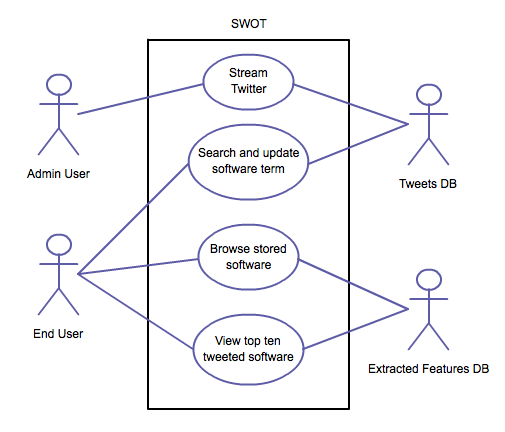
\includegraphics[width=12cm]{uc}
\end{center}
\caption{Use cases for SWOT}
\label{fig:uc}
\end{figure}

\subsection[Use Case 1]{UC1 - Stream Twitter}
\label{sec:uc1}
The first use case for the system requires a tool capable of continuously monitoring public tweets and storing these in a database. These tweets should be filtered by language and relevance, that is, tweets should be related to software. These tweets need to be filtered by language to counter any issues faced in the feature extraction stage due to the complexities involved in NLP. This use case is targetted for use by an administrator as the process should be running constantly in the background.

\subsection[Use Case 2]{UC2 - Search and Update Software Term}
\label{sec:uc2}
SWOT's second use case requires the ability to search Twitter for tweets concerning user-specified key terms. This is ideally the name of some software that may or may not already be present in the database of extracted software and features. In the case where the software is not already present, it will now be added upon finding tweets. Where the software already exists in the database, the search will still be carried out in order to retrieve more recent tweets matching the search query, in order to update the stored data.

\subsection[Use Case 3]{UC3 - Browse Stored Software}
\label{sec:uc3}
The third use case involves allowing users to view the information stored in the database of extracted software and features. This should be displayed in the form of charts displaying the sentiment of tweets and all relevant information found alongside it.

\subsection[Use Case 4]{UC4 - View Top Ten Tweeted Software}
\label{sec:uc4}
The final use case for SWOT requires displaying to users the software tools that have been mentioned most often on Twitter. Users should then also be able to carry out use cases 2 and 3 with these tools.

\section{General Architecture}
The system design follows a 3-stage approach, these being tweet retrieval, feature extraction and visualisation for users. These stages are shown in the general archicture model displayed in Figure~\ref{fig:general}. These will be further explored in Sections~\ref{sec:arc1}, \ref{sec:arc2} and \ref{sec:arc3} respectively.

\begin{figure}[h]
\begin{center}
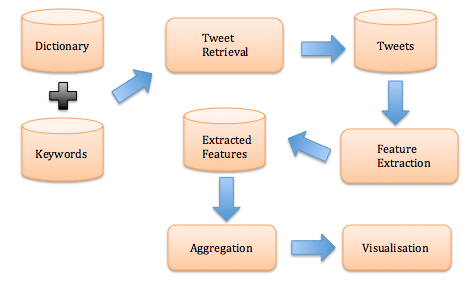
\includegraphics[width=10cm]{design}
\end{center}
\caption{General architecture of the SWOT system}
\label{fig:general}
\end{figure}

\subsection{Retrieving Tweets}
\label{sec:arc1}
The first stage involves retrieving tweets from Twitter. The design for this stage follows the same concepts for each of the use cases defined. This can then be split further as seen in Figure~\ref{fig:phase1}. The program should retrieve a set of search terms from a dictionary along with some keywords that may be associated with software. This dictionary consists of a list of software, companies, operating systems and programming languages. The full list of keywords and dictionary items can be seen in Table~\ref{tbl:keywords} and Appendix~\ref{app:dictionary} respectively. The respective counts for each of these types of items is shown in Table~\ref{tbl:dict_types}.
These are to be used to form a request for tweets from Twitter. Twitter will respond with the corresponding tweets and data, which are to be checked for language, to ensure they are in English. The remaining set of English tweets are then to be further parsed to extract the required information for storing these tweets in the database.

\begin{table}[h]
\begin{center}
\begin{tabular}{|l|l|l|}\hline
alpha&api&app\\\hline
beta&game&mac\\\hline
pc&release&sdk\\\hline
software&source code&version\\\hline
\end{tabular}
\end{center}
\caption{List of keywords}
\label{tbl:keywords}
\end{table}

\begin{table}[h]
\begin{center}
\begin{tabular}{|l|r|}\hline\hline
\textbf{Type}&\textbf{Count}\\\hline
Software&389\\
Operating System&12\\
Company&25\\
Programming Language&448\\
Keywords&12\\\hline
\textbf{Total}&\textbf{886}\\\hline\hline
\end{tabular}
\end{center}
\caption{Number of terms for dictionary types}
\label{tbl:dict_types}
\end{table}

\begin{figure}[h]
  \centering
  \setlength{\unitlength}{0.0125in}
\begin{picture}(300,35)(95,730)
\thicklines
\put(0,740){\framebox(75,20){Filter terms}}
\put(75,750){\vector( 1, 0){ 20}}
\put(95,740){\framebox(75,20){Twitter API}}
\put(170,750){\vector( 1, 0){ 20}}
\put(190,740){\framebox(110,20){Language detection}}
\put(300,750){\vector( 1, 0){ 20}}
\put(320,740){\framebox(80,20){Parse response}}
\put(400,750){\vector( 1, 0){ 20}}
\put(420,740){\framebox(75,20){Store in DB}}
\end{picture}

  \caption{Design for tweet retrieval
    \label{fig:phase1}}
\end{figure}

This returned information will be stored in a relational database and its design is shown below in Figure~\ref{fig:db}. Tweets will not be stored alone but also with simple user information to allow for future user profiling for a more targetted approach to tweet retrieval. The actual tweet information to be stored is its id on the Twitter platform - allowing for cases where users delete their tweets - its text content, time of creation, user id and the keyword used to find it, where one was used. There will also be fields for sentiment, i.e. positive, negative or neutral, and sentiment strength, where weightings have been used. These fields should default to \texttt{NULL} as their values will be computed at a later time. Finally, there is a \emph{tagged} boolean flag which signifies the given tweet has been processed, and the feature extraction process has been carried out on it. This is to work in conjunction with the \emph{found} boolean flag which indicates whether or not software has been found in the tweet. This is to be implemented in MySQL due to its simplicity, compatibility with the design and also because it is readily available on the university computers where data can be easily accessed both locally and remotely.

\begin{figure}[h]
\begin{center}
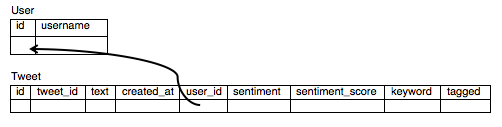
\includegraphics[width=12cm]{db}
\end{center}
\caption{Database design for storing tweets}
\label{fig:db}
\end{figure}

\subsection{Feature Extraction}
\label{sec:arc2}
The feature extraction stage will execute the task of extracting information from tweets. The aim at this stage is to extract the following features:

\begin{itemize}
\item \textbf{Software name} - This discovery is the main purpose of the project and as such is vital.
\item \textbf{Software version} - The version of the software is important because major changes may have been made over the course of a few releases, and so it is necessary to note which release people are referring to.
\item \textbf{Company name} -  This is not a major feature, however it may be interesting to know who developed a certain piece of software. It may also be used where a user of the system wishes to find public sentiment towards a company as opposed to some specific software.
\item \textbf{Programming language} - This feature ideally signifies the language or languages in which the found software was developed. However, as with the company field, this may be used to find sentiment towards specific programming languages or practices.
\item \textbf{Operating system} - Operating system (OS) extraction works similarly to company and programming language extraction in that its expected use is to find the operating systems upon which the found software runs, but it can also be used to find the sentiment towards a specific OS.
\item \textbf{Price} - This is geared towards retrieving information about the user.
\item \textbf{Relevant URLs} - URLs are also extracted for extra information.
\item \textbf{Tweet sentiment} - This is another important feature in terms of the overall project goals. The tweet sentiment aims to find the general sentiment towards a piece of software in a tweet. This will also be used in the final aggregation stages when trying to establish public perception of the software.
\end{itemize}

Extracting these features will involve the stages described in \ref{sec:textmining} and the general design of this process can be seen in Figure~\ref{fig:phase2}. 

\begin{figure}[h]
  \centering
  \setlength{\unitlength}{0.0125in}
\begin{picture}(300,200)( 50, 0)
\thicklines
\put(0,140){\framebox(110,20){Sentiment analysis}}
\put(110,150){\vector( 1, 0){ 20}}
\put(130,140){\framebox(100,20){URL extraction}}
\put(170,750){\line( 1, 0){ 10}}
\put(180,750){\line(0,-1){50}}

\put(300,750){\vector( 1, 0){ 20}}
\put(400,750){\vector( 1, 0){ 20}}



\put(130,140){\framebox(100,20){Price extraction}}
\put(130,140){\framebox(100,20){POS Tagging}}
\put(130,140){\framebox(100,20){Main features}}
\put(130,140){\framebox(100,20){Verify software}}


\end{picture}

  \caption{Design for feature extraction
    \label{fig:phase2}}
\end{figure}

Tweets will be analysed for sentiment after they have been retrieved from the tweet database. This is to be done using the Sentiment140 API, as previously discussed in Section~\ref{sec:back_sent}. As this is a bulk classification service, analysis is to be done on all the tweets retrieved at once, as opposed to individual tweets. This may seem inefficient in the sense that a tweet may be analysed even if it does not contain any references to software. However, using the bulk classification service allows the total number of web requests to be greatly reduced, thus also reducing the overhead when making each request. This will ultimately improve the efficiency of the system.

After this step, URLs need to be extracted from each tweet. URLs provided in tweets related to software are likely to link to further reviews or the application's download page. These should then be removed from the text before further processing as it may cause conflicts when extracting other features.

The text should then be tokenised in order to produce a list of tokens upon which the remaining processing will take place. Prices are the next feature to be extracted. The tokenisation process itself should be able to isolate prices of the form \emph{£10} or \emph{\$0.99} and so this stage will not require much extra processing of the text.

After extracting these two features, the tokens are to be tagged for their part of speech. This will allow for improved entity recognition as linguistic patterns may be applied to the extraction process. The main feature extraction stage has the task of extracting all of the remaining features detailed above. This will require n-gram modelling and linguistic rules and patterns to be able to find candidates for software and other key entities in the text.

These candidates must be verified. If they belong in the dictionary, this is sufficient. However, in cases where the candidate is a new item, other means of verification are required. To do this, SWOT will use the Microsoft Bing API to query the web for these candidates. If the results suggest said candidate is in fact a piece of software, the system will tag these names as software and store the extracted features. In other cases, these features will be discarded.

Due to the volatile nature of the information being extracted from these tweets, this data should be stored in a MongoDB database. As a result, there is no formal design for this database structure, however, it is required of the system to at this stage store any features it has managed to extract along with the key information associated with the tweet that had been stored in the tweet retrieval stage, such as its unique id and text content.

\subsection{Aggregation and Visualisation}
\label{sec:arc3}
The visualisation stage has the task of displaying all the gained information and knowledge to the user. Ultimately, it must also provide a graphical interface for users to interact with the system in order to perform their own searches.

There are two parts to this phase of project. Firstly, the data gathered must be \emph{aggregated} so that meaningful knowledge can ultimately be represented. Upon completing this task, a \emph{graphical user interface} must be designed for users to interact with the system, perform their own queries, and look at what information has been found.

\subsubsection{Aggregation}
Aggregating the results is the process of bringing together all of the different data sources for data on a single output entity such as a piece of software. This aggregated data can then be used easily by the GUI to display information to the user. In this project, this task will entail grouping the stored documents by software or other similar information such as company or operating system. Once this information has been retrieved, statistics and charts can be derived. The main task here is to create pie charts for each piece of software to show the sentiment of the tweets mentioning them. Other details include the most tweeted pieces of software.

\subsubsection{Graphical User Interface}
\label{sec:guid}
Upon the completion of the aggregation tasks, these charts and statistics need to be passed to a Graphical User Interface (GUI). The GUI of choice for this system is a web application, as opposed to a desktop application. This is a more extensible solution as changes would not need to be pushed out to all users.

There will be three actions for users to carry out on this GUI. These will relate to use case 2 of this system, as seen in Section~\ref{sec:uc2}. The first action to carry out will be searching for tweets posted on Twitter. A mockup of this action can be seen in Figure~\ref{fig:guiwire2}. Once these tweets have been retrieved from the Twitter Search API, they will be displayed on the web page, and in turn features will be extracted, and again displayed to the user.

After this, there will be an analysis page. This page will show a list of software or operating systems, from which a user can select to view charts displaying sentiment and a list of tweets. These charts will have been creating in the aggregation stage, but should be dynamically created. This page is shown in Figure~\ref{fig:guiwire3}.

Finally, once a number of tools, that is, software, operating systems etc. have been found in tweets, the home page should display a list of the most tweeted of these items. Clicking on an item in this list should offer the option of searching again for it, in order to update information, or to view its charts and sentiment information. This should look as the wireframe in Figure~\ref{fig:guiwire1}.

\begin{figure}[h]
\begin{center}
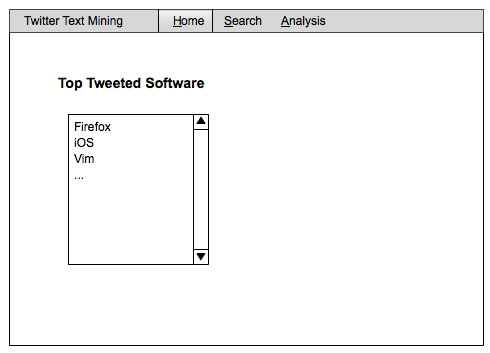
\includegraphics[width=10cm]{guiwire1}
\end{center}
\caption{A mockup of the website's home page}
\label{fig:guiwire1}
\end{figure}

\begin{figure}[h]
\begin{center}
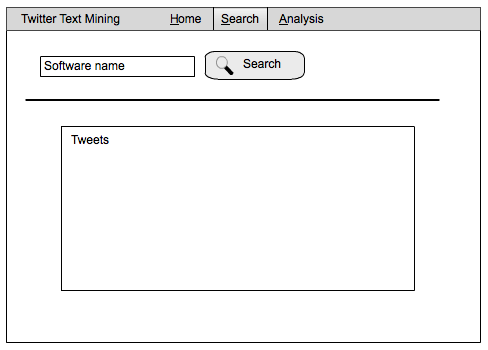
\includegraphics[width=10cm]{guiwire2}
\end{center}
\caption{A mockup of the website's search page}
\label{fig:guiwire2}
\end{figure}

\begin{figure}[h]
\begin{center}
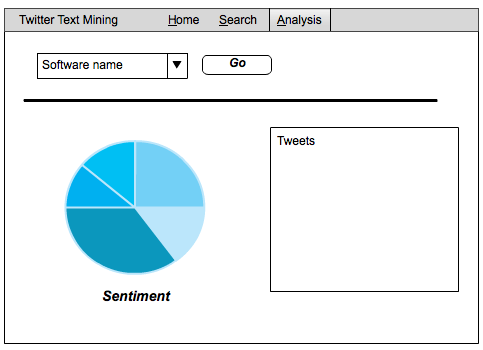
\includegraphics[width=10cm]{guiwire3}
\end{center}
\caption{A mockup of the website's analysis page}
\label{fig:guiwire3}
\end{figure}

